% Options for packages loaded elsewhere
% Options for packages loaded elsewhere
\PassOptionsToPackage{unicode}{hyperref}
\PassOptionsToPackage{hyphens}{url}
\PassOptionsToPackage{dvipsnames,svgnames,x11names}{xcolor}
%
\documentclass[
  letterpaper,
  enabledeprecatedfontcommands]{report}
\usepackage{xcolor}
\usepackage[top=2cm,left=2cm,right=5cm]{geometry}
\usepackage{amsmath,amssymb}
\setcounter{secnumdepth}{5}
\usepackage{iftex}
\ifPDFTeX
  \usepackage[T1]{fontenc}
  \usepackage[utf8]{inputenc}
  \usepackage{textcomp} % provide euro and other symbols
\else % if luatex or xetex
  \usepackage{unicode-math} % this also loads fontspec
  \defaultfontfeatures{Scale=MatchLowercase}
  \defaultfontfeatures[\rmfamily]{Ligatures=TeX,Scale=1}
\fi
\usepackage{lmodern}
\ifPDFTeX\else
  % xetex/luatex font selection
  \setmainfont[]{Helvetica}
\fi
% Use upquote if available, for straight quotes in verbatim environments
\IfFileExists{upquote.sty}{\usepackage{upquote}}{}
\IfFileExists{microtype.sty}{% use microtype if available
  \usepackage[]{microtype}
  \UseMicrotypeSet[protrusion]{basicmath} % disable protrusion for tt fonts
}{}
\makeatletter
\@ifundefined{KOMAClassName}{% if non-KOMA class
  \IfFileExists{parskip.sty}{%
    \usepackage{parskip}
  }{% else
    \setlength{\parindent}{0pt}
    \setlength{\parskip}{6pt plus 2pt minus 1pt}}
}{% if KOMA class
  \KOMAoptions{parskip=half}}
\makeatother
% Make \paragraph and \subparagraph free-standing
\makeatletter
\ifx\paragraph\undefined\else
  \let\oldparagraph\paragraph
  \renewcommand{\paragraph}{
    \@ifstar
      \xxxParagraphStar
      \xxxParagraphNoStar
  }
  \newcommand{\xxxParagraphStar}[1]{\oldparagraph*{#1}\mbox{}}
  \newcommand{\xxxParagraphNoStar}[1]{\oldparagraph{#1}\mbox{}}
\fi
\ifx\subparagraph\undefined\else
  \let\oldsubparagraph\subparagraph
  \renewcommand{\subparagraph}{
    \@ifstar
      \xxxSubParagraphStar
      \xxxSubParagraphNoStar
  }
  \newcommand{\xxxSubParagraphStar}[1]{\oldsubparagraph*{#1}\mbox{}}
  \newcommand{\xxxSubParagraphNoStar}[1]{\oldsubparagraph{#1}\mbox{}}
\fi
\makeatother


\usepackage{longtable,booktabs,array}
\usepackage{calc} % for calculating minipage widths
% Correct order of tables after \paragraph or \subparagraph
\usepackage{etoolbox}
\makeatletter
\patchcmd\longtable{\par}{\if@noskipsec\mbox{}\fi\par}{}{}
\makeatother
% Allow footnotes in longtable head/foot
\IfFileExists{footnotehyper.sty}{\usepackage{footnotehyper}}{\usepackage{footnote}}
\makesavenoteenv{longtable}
\usepackage{graphicx}
\makeatletter
\newsavebox\pandoc@box
\newcommand*\pandocbounded[1]{% scales image to fit in text height/width
  \sbox\pandoc@box{#1}%
  \Gscale@div\@tempa{\textheight}{\dimexpr\ht\pandoc@box+\dp\pandoc@box\relax}%
  \Gscale@div\@tempb{\linewidth}{\wd\pandoc@box}%
  \ifdim\@tempb\p@<\@tempa\p@\let\@tempa\@tempb\fi% select the smaller of both
  \ifdim\@tempa\p@<\p@\scalebox{\@tempa}{\usebox\pandoc@box}%
  \else\usebox{\pandoc@box}%
  \fi%
}
% Set default figure placement to htbp
\def\fps@figure{htbp}
\makeatother





\setlength{\emergencystretch}{3em} % prevent overfull lines

\providecommand{\tightlist}{%
  \setlength{\itemsep}{0pt}\setlength{\parskip}{0pt}}



 


\makeatletter
\@ifpackageloaded{tcolorbox}{}{\usepackage[skins,breakable]{tcolorbox}}
\@ifpackageloaded{fontawesome5}{}{\usepackage{fontawesome5}}
\definecolor{quarto-callout-color}{HTML}{909090}
\definecolor{quarto-callout-note-color}{HTML}{0758E5}
\definecolor{quarto-callout-important-color}{HTML}{CC1914}
\definecolor{quarto-callout-warning-color}{HTML}{EB9113}
\definecolor{quarto-callout-tip-color}{HTML}{00A047}
\definecolor{quarto-callout-caution-color}{HTML}{FC5300}
\definecolor{quarto-callout-color-frame}{HTML}{acacac}
\definecolor{quarto-callout-note-color-frame}{HTML}{4582ec}
\definecolor{quarto-callout-important-color-frame}{HTML}{d9534f}
\definecolor{quarto-callout-warning-color-frame}{HTML}{f0ad4e}
\definecolor{quarto-callout-tip-color-frame}{HTML}{02b875}
\definecolor{quarto-callout-caution-color-frame}{HTML}{fd7e14}
\makeatother
\makeatletter
\@ifpackageloaded{bookmark}{}{\usepackage{bookmark}}
\makeatother
\makeatletter
\@ifpackageloaded{caption}{}{\usepackage{caption}}
\AtBeginDocument{%
\ifdefined\contentsname
  \renewcommand*\contentsname{Table of contents}
\else
  \newcommand\contentsname{Table of contents}
\fi
\ifdefined\listfigurename
  \renewcommand*\listfigurename{List of Figures}
\else
  \newcommand\listfigurename{List of Figures}
\fi
\ifdefined\listtablename
  \renewcommand*\listtablename{List of Tables}
\else
  \newcommand\listtablename{List of Tables}
\fi
\ifdefined\figurename
  \renewcommand*\figurename{Figure}
\else
  \newcommand\figurename{Figure}
\fi
\ifdefined\tablename
  \renewcommand*\tablename{Table}
\else
  \newcommand\tablename{Table}
\fi
}
\@ifpackageloaded{float}{}{\usepackage{float}}
\floatstyle{ruled}
\@ifundefined{c@chapter}{\newfloat{codelisting}{h}{lop}}{\newfloat{codelisting}{h}{lop}[chapter]}
\floatname{codelisting}{Listing}
\newcommand*\listoflistings{\listof{codelisting}{List of Listings}}
\makeatother
\makeatletter
\makeatother
\makeatletter
\@ifpackageloaded{caption}{}{\usepackage{caption}}
\@ifpackageloaded{subcaption}{}{\usepackage{subcaption}}
\makeatother
\usepackage{bookmark}
\IfFileExists{xurl.sty}{\usepackage{xurl}}{} % add URL line breaks if available
\urlstyle{same}
\hypersetup{
  colorlinks=true,
  linkcolor={blue},
  filecolor={Maroon},
  citecolor={Blue},
  urlcolor={Blue},
  pdfcreator={LaTeX via pandoc}}


\author{}
\date{}
\begin{document}

\renewcommand*\contentsname{Table of contents}
{
\hypersetup{linkcolor=}
\setcounter{tocdepth}{2}
\tableofcontents
}

\bookmarksetup{startatroot}

\chapter*{Welcome to the Complex Disordered Matter
Course!}\label{welcome-to-the-complex-disordered-matter-course}
\addcontentsline{toc}{chapter}{Welcome to the Complex Disordered Matter
Course!}

\markboth{Welcome to the Complex Disordered Matter Course!}{Welcome to
the Complex Disordered Matter Course!}

\pandocbounded{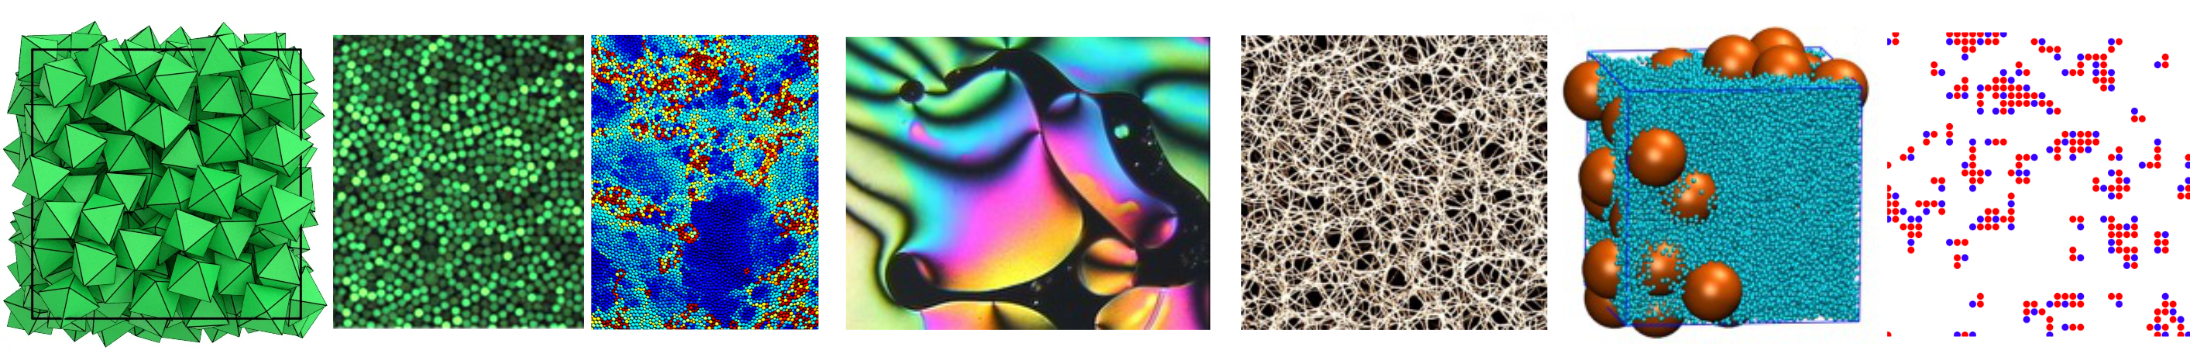
\includegraphics[keepaspectratio]{placeholder_figure_long.png}}\hfill

\section*{Overview}\label{overview}
\addcontentsline{toc}{section}{Overview}

\markright{Overview}

This course introduces your to the theoretical, computational and
experimental aspects of the physics of complex disordered matter.

Complex disordered matter is the study of wide range of systems like
\textbf{polymers}, \textbf{colloids}, \textbf{glasses}, \textbf{gels},
and \textbf{emulsions}, which lack long-range order but exhibit
intricate behaviour. Colloids, suspensions of microscopic particles in a
fluid, are useful for studying disordered structures due to their
observable dynamics. Similarly, polymer systems can form amorphous
solids or glasses when densely packed or cooled, showing solid-like
rigidity despite their disordered structure. These materials often
undergo phase transitions, such as demixing and crystallisation, and
near these transitions, they can display critical phenomena with
extensive fluctuations and correlations.

These various are examples of \textbf{soft matter}. systems In soft
matter systems, the interplay between disorder, softness, and phase
behavior leads to rich physical phenomena, particularly near critical
points where even small changes in external conditions can trigger
large-scale reorganizations and universal behaviour. Glasses, for
instance, exhibit slow relaxation and memory effects, while colloidal
systems may crystallize, phase separate, or become jammed depending on
particle interactions and concentration. Understanding such behaviors
involves studying how microscopic interactions and thermal fluctuations
influence macroscopic properties, especially in non-equilibrium
conditions. Through techniques like scattering, microscopy, rheology,
and simulation, one can explore how disordered soft materials respond to
stress, age, or undergo transitions---insights that are vital for
applications in materials design, biotechnology, and beyond.

This course is organized into three interconnected parts, each offering
a distinct perspective on the study of complex disordered matter.

\begin{itemize}
\tightlist
\item
  \textbf{Part 1: Unifying concepts} (Nigel Wilding) introduces the
  theoretical framework for rationalising complex disordered matter
  which is grounded in statistical mechanics and thermodynamics. We
  emphasize the theory of phase transitions, thermal fluctuations,
  critical phenomena, and stochastic dynamics---providing the essential
  theoretical tools needed to describe and predict the behavior of soft
  and disordered systems.\\
\item
  \textbf{Part 2: Complex disordered matter} (Francesco Turci) explores
  the phenomenology of key examples of complex disordered soft matter
  systems, including colloids, polymers, liquid crystals, glasses, gels,
  and active matter. These systems will be analyzed using the
  theoretical concepts introduced in Part 1, highlighting how disorder,
  interactions, and fluctuations shape their macroscopic behavior.\\
\item
  \textbf{Part 3: Experimental techniques} (Adrian Barnes) focuses on
  the methods of microscopy, and scattering via x-rays, neutrons and
  light that are used to study complex disordered matter, offering
  insight into how their properties are measured and understood in
  real-world contexts.
\end{itemize}

In addition to theory and experiment, computer simulation plays a
central role in soft matter research. This course includes a substantial
coursework component consisting of two computational projects. These
exercises will allow you to apply state-of-the-art simulation techniques
to investigate the complex behavior of disordered systems, bridging
theory and observation through hands-on exploration.

\section*{Delivery and format}\label{delivery-and-format}
\addcontentsline{toc}{section}{Delivery and format}

\markright{Delivery and format}

\begin{itemize}
\item
  Detailed e-notes (accessible via Blackboard) can be viewed on a
  variety of devices. Pdf is also available.
\item
  We will give `traditional' lectures (Tuesdays, Wednesdays, Fridays) in
  which we use slides to summarise and explain the lecture content.
  Questions are welcome (within reason\ldots)
\item
  Try to read ahead in the notes, then come to lectures, listen to the
  explanations and then reread the notes.
\item
  Rewriting the notes or slides to express your own thoughts and
  understanding, or annotating a pdf copy can help wire the material
  into your own way of thinking.
\item
  There are problem classes (Thursdays) where you can try problem sheets
  and seek help. Lecturers may go over some problems with the class.
\item
  The navigation bar on the left will allow you to access the lecture
  notes and problem sets.
\end{itemize}

\section*{Intended learning outcomes}\label{intended-learning-outcomes}
\addcontentsline{toc}{section}{Intended learning outcomes}

\markright{Intended learning outcomes}

The course will

\begin{itemize}
\tightlist
\item
  Introduce you to the qualitative features of a range of complex and
  disordered systems and the experimental techniques used to study them.
\item
  Introduce you to a range of model systems and theoretical techniques
  used to elucidate the physics of complex disordered matter.
\item
  Provide you with elementary computational tools to model complex
  disordered systems numerically and predict their properties.
\item
  Allow you to apply your physics background to understand a variety of
  systems of inter-disciplinary relevance.
\item
  Connect with the most recent advances in the research on complex
  disordered matter.
\end{itemize}

\section*{Contact details}\label{contact-details}
\addcontentsline{toc}{section}{Contact details}

\markright{Contact details}

The course will be taught by

\begin{itemize}
\tightlist
\item
  Prof Nigel B. Wilding (unit director): nigel.wilding@bristol.ac.uk
\item
  Dr Francesco Turci: F.Turci@bristol.ac.uk
\item
  Dr Adrian Barnes: a.c.barnes@bristol.ac.uk
\end{itemize}

\section*{Questions and comments}\label{questions-and-comments}
\addcontentsline{toc}{section}{Questions and comments}

\markright{Questions and comments}

If you have any questions about the course, please don't hesitate to
contact the relevant lecturer, either by email (see above) or in a
problems class.

Finally, this is a new course for 2025/26. If you find any errors or
mistakes or something which isn't clear, please let us know by email, or
fill in this anonymous form:

\begin{tcolorbox}[enhanced jigsaw, breakable, colback=white, colframe=quarto-callout-note-color-frame, bottomrule=.15mm, leftrule=.75mm, toprule=.15mm, opacityback=0, arc=.35mm, rightrule=.15mm, left=2mm]

\href{https://forms.office.com/e/6uL2Bd5QGq}{Submit an
error/mistake/query}

\end{tcolorbox}

\bookmarksetup{startatroot}

\chapter*{Unifying concepts: Problems}\label{problems}
\addcontentsline{toc}{chapter}{Unifying concepts: Problems}

\markboth{Unifying concepts: Problems}{Unifying concepts: Problems}

Although you should try all of these questions, some of them are
deliberately quite challenging. If you don't get very far with some,
don't worry. We'll be going over them in problems classes, so you can
just regard them as worked examples.

\subsection*{\texorpdfstring{1. Existence of a phase transition in
\(d=2\).}{1. Existence of a phase transition in d=2.}}\label{existence-of-a-phase-transition-in-d2.}
\addcontentsline{toc}{subsection}{1. Existence of a phase transition in
\(d=2\).}

In lectures it was argued that no long ranged order occurs at
finite-temperatures in a one dimensional system because of the presence
of domain walls. Were macroscopic domain walls to exist in two
dimensions at finite temperature, they would similarly destroy long
ranged order and prevent a phase transition. By calculating the free
energy of a 2D domain wall for an Ising lattice, show that domain walls
do not in fact exist for sufficiently low \(T\).

(Hint: Model the domain wall as a non-reversing \(N\)-step random walk
on the lattice and find an expression for its energy and -from the
number of random walk configurations- its entropy.)

\begin{center}\rule{0.5\linewidth}{0.5pt}\end{center}

\subsection*{2. Correlation Length}\label{correlation-length}
\addcontentsline{toc}{subsection}{2. Correlation Length}

For a 1D Ising model, show that the correlation between the spins at
sites \(i\) and \(j\), is

\[\langle s_i s_j\rangle =\sum_m p_m(-1)^m\] where \(m\) is the number
of domain walls between \(i\) and \(j\) and \(p_m\) is the probability
of finding \(m\) domain walls between them.

Hence show that when \(R_{ij}=|i-j|a\) is large (with \(a\) the lattice
spacing) and the temperature is small, that

\[\langle s_i s_j\rangle =\exp(-R_{ij}/\xi)\] with \(\xi=a/2p\) and
\(p\) the probability of finding a domain wall on a bond.

\emph{Hint: In the second part note that \(p_m\) is given by a binomial
distribution because there is a probability \(p\) of each bond
containing a domain wall and \((1-p)\) that it doesn't. What special
type of distribution does \(p_m\) tend to when \(p\) is small (as occurs
at low \(T\))?}

\begin{center}\rule{0.5\linewidth}{0.5pt}\end{center}

\subsection*{3. A model fluid}\label{a-model-fluid}
\addcontentsline{toc}{subsection}{3. A model fluid}

The van der Waals (vdW) equation of state is essentially a mean field
theory for fluids. It relates the pressure and the volume of a fluid to
the temperature:

\[\left(P+\frac{a}{V^2}\right)(V-b)=N_Ak_BT\] where \(a\) and \(b\) are
constants and \(N_A\) is Avogadro's number.

The critical point of a fluid corresponds to the point at which the
isothermal compressibility diverges, that is

\[\left(\frac{\partial P}{\partial V}\right)_T=0\] Additionally, one
finds that isotherms of \(P\) versus \(V\) exhibit a point of inflection
at the critical point, that is

\[\left(\frac{\partial^2 P}{\partial V^2}\right)_T=0\]

\begin{itemize}
\item
  Use these two requirements to show that the critical point of the vdW
  fluid is located at

  \[V_c=3b, ~~~ P_c=\frac{a}{27b^2},~~~ N_AK_BT_c=\frac{8a}{27b}\]
\item
  Hence show that when written in terms of reduced variables

  \[p=\frac{P}{P_c}, ~~~~ v=\frac{V}{V_c} ~~~~ t=\frac{T}{T_c}\]

  the equation takes the form

  \[\left(p+\frac{3}{v^2}\right)(v-\frac{1}{3})=\frac{8t}{3}\]
\item
  Write a Python script to plot a selection of isotherms close to the
  critical temperature (you will need to choose suitable units for your
  axes). Plot also the gradient and second derivative of \(P\) vs \(V\)
  on the critical isotherm and confirm numerically that it exhibits a
  point of inflection at the critical pressure and temperature.
\item
  Obtain the value of the critical exponent \(\gamma\) of the vdW model
  and confirm that it takes a mean-field value.
\end{itemize}

\begin{center}\rule{0.5\linewidth}{0.5pt}\end{center}

\subsection*{4. Mean field theory of the Ising model heat
capacity}\label{mean-field-theory-of-the-ising-model-heat-capacity}
\addcontentsline{toc}{subsection}{4. Mean field theory of the Ising
model heat capacity}

Using results derived in lectures, obtain an expression for the mean
energy \(\langle E\rangle\) of the Ising model in zero field, within the
simplest mean field approximation \(\langle
  s_is_j\rangle=\langle s_i\rangle\langle s_j\rangle=m^2\). Hence show
that for \(H=0\) the heat capacity \(\partial \langle
  E\rangle/\partial T\) has the behaviour \[
\begin{eqnarray*}
C_H&=& 0 ~~~~ T>T_c\\
C_H&=& 3Nk_B/2 ~~~~ T\le T_c
\end{eqnarray*}
\]

\begin{center}\rule{0.5\linewidth}{0.5pt}\end{center}

\subsection*{5. Magnetisation and
fluctuations}\label{magnetisation-and-fluctuations}
\addcontentsline{toc}{subsection}{5. Magnetisation and fluctuations}

A system of spins on a lattice, has, in the absence of an applied field,
a Hamiltonian \({\cal H}\). In the presence of a field \(h\) the
Hamiltonian becomes \[
\tilde {\cal H}={\cal H}-hM
\] where \(M\) is the total magnetisation and \(h\) is the magnetic
field. By considering the partition function \(Z(T,h)\) and its
relationship to the free energy \(F\) show that in general

\[
\langle M \rangle=-\left(\frac{\partial F}{\partial h}\right)_T
\]

Show also that the variance of the magnetisation fluctuations is

\[\langle M^2\rangle-\langle M\rangle^2=-k_BT\left(\frac{\partial^2 F}{\partial h^2}\right)_T\]

(\emph{Hint: This is an important standard derivation found in many text
books on Statistical Mechanics. You will need to differentiate \(F\)
(twice) and use the product and chain rules.})

\begin{center}\rule{0.5\linewidth}{0.5pt}\end{center}

\subsection*{6. Spin-1 Ising model}\label{spin-1-ising-model}
\addcontentsline{toc}{subsection}{6. Spin-1 Ising model}

A set of spins on a lattice of coordination number \(q\) can take values
\((-1,0,1)\), as opposed to just \((-1,1)\) as in the spin-1/2 Ising
model. The Hamiltonian is

\[{\cal H}=-J\sum_{<ij>}s_is_j + h\sum_i s_i\]

Find the partition function and hence show that in the mean field
approximation, the magnetisation per site obeys

\[m=\frac{2\sinh[\beta(Jqm+h)]}{2\cosh[\beta(Jqm+h)]+1}\]

and find the critical temperature \(T_c\) at which the net magnetisation
vanishes.

\begin{center}\rule{0.5\linewidth}{0.5pt}\end{center}

\subsection*{7. Transfer Matrix.}\label{transfer-matrix.}
\addcontentsline{toc}{subsection}{7. Transfer Matrix.}

Verify the calculation of the free energy of the 1D periodic chain Ising
model in a field outlined in lectures using the Transfer Matrix method.

Use your results to show that the spontaneous magnetisation is:

\[m=\frac{\sinh \beta H}{\sqrt{\sinh^2\beta H+\exp{-4\beta J}}}\]
Comment on the value of \(m\) in zero field.

(\emph{Hint: Follow the prescription given in lectures. Depending on
your approach you may need to use the trigonometrical identities
\(\cosh^2x-\sinh^2x=1\), \(\cosh(2x)=2\cosh^2x-1\).})

\begin{center}\rule{0.5\linewidth}{0.5pt}\end{center}

\subsection*{8. Landau theory}\label{landau-theory}
\addcontentsline{toc}{subsection}{8. Landau theory}

Check and complete the Landau theory calculations, given in lectures,
for the critical exponents \(\gamma=1\) and \(\alpha=0\) of the Ising
model. For the latter, you should first prove the result

\[C_H =-T\frac{\partial^2 F}{\partial T^2}\] starting from the classical
theormodynamics expression for changes in the free energy of a magnet
\(dF=-SdT-MdH\).

(\emph{Hint: If you get stuck with the proof see standard thermodynamics
text books. To get the susceptibility exponent in Landau theory add a
term \(-Hm\) to the Hamiltonian.})

\begin{center}\rule{0.5\linewidth}{0.5pt}\end{center}

\subsection*{9. Scaling equation of
state}\label{scaling-equation-of-state}
\addcontentsline{toc}{subsection}{9. Scaling equation of state}

Consider a Landau expression for the free energy of a magnetic system
having magnetisation \(m\):

\[
F=F_0+\tilde{a}_2tm^2+a_4m^4-Hm\:,
\] where \(t=T-T_c\) and \(H\) is an applied magnetic field;
\(\tilde{a}_2\) and \(a_4\) are positive constants and \(F_0\) is a
constant background term.

Show that the equation of state for the model is

\[
H=2\tilde{a}_2tm+4a_4m^3\:.
\]

Use the near-critical power law behaviour of \(m\) to show that the
equation of state may be written in the scaling form

\[
\frac{H}{m^\delta}=g\left(\frac{t}{m^{1/\beta}}\right)\:,
\] and find the (mean field) values of the critical exponents \(\delta\)
and \(\beta\).

Deduce that \(g(x)=x+1\) up to a choice of scale for \(\tilde{a}_2\) and
\(a_4\).

\begin{center}\rule{0.5\linewidth}{0.5pt}\end{center}

\subsection*{10. Scaling laws}\label{scaling-laws}
\addcontentsline{toc}{subsection}{10. Scaling laws}

Using the generalised homogeneous form for the free energy given in
lectures, take appropriate derivatives to find the relationships to the
critical exponents:

\[
\beta=\frac{1-b}{a}; ~~ \gamma=\frac{2b-1}{a};~~ \delta= \frac{b}{1-b}; ~~~ \alpha=2-\frac{1}{a}.
\]

Hence derive the scaling laws among the critical exponents: \[
\begin{eqnarray*}
\alpha+\beta(\delta+1)&=& 2 \\
\alpha+2\beta+\gamma &=& 2\\
%\gamma=\beta(\delta-1)
\end{eqnarray*}\] (\emph{Hint: For the heat capacity exponent \(\alpha\)
use the result from problem 8:
\(C_H=-T\left(\frac{\partial^2F}{\partial T^2}\right)_{h=0}\)})

\begin{center}\rule{0.5\linewidth}{0.5pt}\end{center}

\subsection*{11. Classical nucleation
theory}\label{classical-nucleation-theory}
\addcontentsline{toc}{subsection}{11. Classical nucleation theory}

A supercooled liquid metal is undergoing solidification. According to
classical nucleation theory, the Gibbs free energy change \(\Delta G\)
for forming a spherical solid nucleus of radius \(r\) in the liquid is
given by:

\[
\Delta G(r) = \frac{4}{3}\pi r^3 \Delta G_v + 4\pi r^2 \gamma
\] where \(\Delta G_v < 0\) is the free energy change per unit volume
due to the phase change, and \(\gamma > 0\) is the interfacial energy
between the solid and liquid phases.

\textbf{(a)} Derive the expression for the critical radius \(r^*\) at
which the nucleus becomes stable and begins to grow.

\textbf{(b)} Show that the critical energy barrier for nucleation
\(\Delta G^*\) is given by:

\[
\Delta G^* = \frac{16\pi \gamma^3}{3 (\Delta G_v)^2}
\]

\textbf{(c)} Explain qualitatively how the degree of undercooling
\(\Delta T\) affects the rate of nucleation. You may use the fact that
\(\Delta G_v \propto \Delta T\) to support your answer.

\begin{center}\rule{0.5\linewidth}{0.5pt}\end{center}

\subsection*{12. Colloidal diffusion}\label{colloidal-diffusion}
\addcontentsline{toc}{subsection}{12. Colloidal diffusion}

A large colloidal particle of mass \(M\) moves in a fluid under the
influence of a random force \(F(t)\) and a coefficient of Stokes
friction drag \(\gamma\), both per unit mass. If the solution of the
corresponding Langevin equation for the velocity of the colloidal
particle is given by

\[
u = u_0 e^{-\gamma t} + \frac{e^{-\gamma t}}{M} \int_0^t dt' \, e^{\gamma t'} F(t'),
\]

where \(u_0\) is the velocity at \(t = 0\), show that for long times the
velocity of the particle satisfies the relation

\[
\langle u^2 \rangle = \frac{kT}{M} + \left( u_0^2 - \frac{kT}{M} \right) e^{-2\gamma t},
\]

where \(k\) is the Boltzmann constant and \(T\) is the absolute
temperature.

State clearly any assumptions that you make.

\begin{center}\rule{0.5\linewidth}{0.5pt}\end{center}

\subsection*{13. Einstein's expression for the diffusion
coefficient}\label{einsteins-expression-for-the-diffusion-coefficient}
\addcontentsline{toc}{subsection}{13. Einstein's expression for the
diffusion coefficient}

In 1905, Einstein showed that the friction coefficient \(\gamma\) (per
unit mass) of a colloidal particle must be related to the diffusion
coefficient \(D\) of the particle by

\[
D = \frac{kT}{\gamma}.
\]

If a marked particle covers a distance \(X\) in a given time \(t\)
(assuming a one-dimensional random walk), the diffusion coefficient is
defined to be

\[
D = \lim_{t \to \infty} \frac{1}{2t} \langle [X(t) - X(0)]^2 \rangle,
\]

where the average \(\langle \cdot \rangle\) is taken over an ensemble in
thermal equilibrium.

Use the fact that \(X(t) - X(0)
= \int_{0}^{t} u(t')\,\mathrm{d}t'\) to show that the Einstein relation
may be written as

\[
\gamma = \frac{1}{\mu} = \frac{D}{kT} = \frac{1}{kT} \int_0^\infty \langle u(t_0) u(t_0 + t) \rangle \, dt,
\]

where \(\mu\) is known as the mobility of the particle and \(t_0\) is
any arbitrarily chosen time.

\begin{center}\rule{0.5\linewidth}{0.5pt}\end{center}

\subsection*{14. Life in one dimension}\label{life-in-one-dimension}
\addcontentsline{toc}{subsection}{14. Life in one dimension}

A particle lives on the sites of a one-dimensional lattice. At any
instant it has probability \(\alpha\) per unit time that it will hop to
the site on its right and probability \(\alpha\) per unit time of
hopping to the site on its left.

Write down the master equation for the set of probabilities \(p_n(t)\)
of finding the particle at the \(n^{\text{th}}\) site, where
\(-\infty < n < \infty\).

Solve the master equation for the \(p_n\), subject to the initial
condition that the particle was at the site \(n = 0\) at time \(t = 0\).
Hence obtain the mean position \(\langle n \rangle\) and root mean
square deviation from the mean, both as functions of time.

\textbf{Hint}: The second part of the question is most easily done by
introducing the generating function

\[
F(z, t) = \sum_{n=-\infty}^{\infty} p_n(t) z^n.
\]

\begin{center}\rule{0.5\linewidth}{0.5pt}\end{center}

\subsection*{15. Master equation}\label{master-equation}
\addcontentsline{toc}{subsection}{15. Master equation}

A system of \(N\) atoms, each having two energy levels
\(E = \pm \epsilon\), is brought into contact with a heat bath at
temperature \(T\). The atoms do not interact with each other, but each
atom interacts with the heat bath to have a probability
\(\lambda_{-\to+}(T)\) per unit time of transition from lower to higher
level, and a probability \(\lambda_{+\to-}(T)\) per unit time of the
reverse transition.

If at any time \(t\) there are \(n_+(t)\) atoms at the higher level and
\(n_-(t)\) at the lower level, then \(n(t) = n_-(t) - n_+(t)\) is a
convenient measure of the non-equilibrium state.

Obtain the master equation for \(n(t)\) and hence the relaxation time
\(\tau\) which characterizes the exponential approach of the system to
equilibrium.

\begin{center}\rule{0.5\linewidth}{0.5pt}\end{center}

\subsection*{16. Detailed balance}\label{detailed-balance}
\addcontentsline{toc}{subsection}{16. Detailed balance}

\textbf{(a)} Starting from the principle of detailed balance for an
isolated system, show that for two groups of states within it, \(A\) and
\(B\), the overall rate of transitions from group \(A\) to group \(B\)
is balanced, in equilibrium, by those from \(B\) to \(A\):

\[
\lambda_{A \to B} p^{\text{eq}}_A = \lambda_{B \to A} p^{\text{eq}}_B
\]

\textbf{(b)} Deduce that the principle applies to microstates in the
canonical ensemble, and hence that the jump rates between states of a
subsystem (of fixed number of particles) connected to a heat bath must
obey

\[
\frac{\lambda_{i \to j}}{\lambda_{j \to i}} = e^{-(E_j - E_i)/kT}.
\]

\begin{center}\rule{0.5\linewidth}{0.5pt}\end{center}

\subsection*{17. Jump processes}\label{jump-processes}
\addcontentsline{toc}{subsection}{17. Jump processes}

An isolated system can occupy three possible states of the same energy.
The kinetics are such that it can jump from state 1 to 2 and 2 to 3 but
not directly from 1 to 3. Per unit time, there is a probability
\(\lambda_0\) that the system makes a jump, from the state it is in,
into (each of) the other state(s) it can reach.

\textbf{(a)} Show that the occupancy probabilities
\(p = (p_1, p_2, p_3)\) of the three states obey the master equation

\[
\dot{p} = M \cdot p
\]

where the rate matrix is

\[
M = \lambda_0 \begin{bmatrix}
-1 & 1 & 0 \\
1 & -2 & 1 \\
0 & 1 & -1
\end{bmatrix}
\]

\textbf{(b)} Confirm that an equilibrium state is \(p = (1, 1, 1)/3\).

\textbf{(c)} Prove this equilibrium state is unique.

\textbf{Hint}: For part (c), consider the eigenvalues of \(M\).




\end{document}
